\section{Implementation}

\begin{frame}{Atari Wrappers}
    Atari wrappers from OpenAI baselines:
    \begin{itemize}
    \item \texttt{EpisodicLifeEnv}: make an ``end of life'' be the end
        of the episode resetting the environment only on the true
        game over, this helps in value estimation
    \item \texttt{FireResetEnv}: use ``Fire'' as starting action in order
        to launch the ball
    \item \texttt{MaxAndSkipEnv}: returns only the skip-th frame, this
        reduces the amount of frame the agent has to deal with (set to 4
        in the main experiments)
\end{itemize}
\end{frame}

\begin{frame}{Robot Features Extraction}
    \begin{itemize}
        \item extracting \textbf{paddle position}
        \item extracting \textbf{ball position}
        \item features can be increased with \textbf{ball direction}
        \item \textbf{previous positions} could help the training too
        \item more features increase the state space
        \item OpenCV
    \end{itemize}
\end{frame}

\begin{frame}{Robot Features Extraction}
    \begin{columns}[c,onlytextwidth]
        \column{0.7\textwidth}
            \parbox{0.95\textwidth}{
                Extracting \textbf{paddle position} from the
                observation: tensor of dimension $(210, 160, 3)$
                where each value represents a color of the pixel.
            }
        \column{0.3\textwidth}
            \begin{figure}
                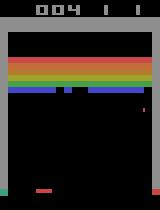
\includegraphics[width=\textwidth]{images/robotfeaturesextractorsequence/robotfeatures-original-image.jpg}
            \end{figure}
    \end{columns}
\end{frame}

\begin{frame}{Robot Features Extraction}
    \begin{columns}[c,onlytextwidth]
        \column{0.7\textwidth}
            \parbox{0.95\textwidth}{
                Considering only the \textbf{lower part} of the\\
                observation which contains the paddle.}
        \column{0.3\textwidth}
            \begin{figure}
                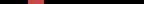
\includegraphics[width=\textwidth]{images/robotfeaturesextractorsequence/robotfeatures-bottom-part.jpg}
            \end{figure}
    \end{columns}
\end{frame}

\begin{frame}{Robot Features Extraction}
    \begin{columns}[c,onlytextwidth]
        \column{0.7\textwidth}
            \parbox{0.95\textwidth}{
                Converting the image to \textbf{gray-scale} in order to
                reduce the number of channels.

                This makes it easier to apply a threshold \mbox{function}.
            }
        \column{0.3\textwidth}
            \begin{figure}
                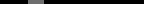
\includegraphics[width=\textwidth]{images/robotfeaturesextractorsequence/robotfeatures-bottom-part-gray.jpg}
            \end{figure}
    \end{columns}
\end{frame}

\begin{frame}{Robot Features Extraction}
    \begin{columns}[c,onlytextwidth]
        \column{0.7\textwidth}
            Determine the position of the paddle:
            \begin{itemize}
                \item apply a \textbf{threshold} function to obtain a black and white image
                \item find \textbf{contours}
                \item extract \textbf{centroid} of the paddle
                \item $\text{paddle}_x=35$
            \end{itemize}
        \column{0.3\textwidth}
            \begin{figure}
                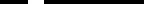
\includegraphics[width=\textwidth]{images/robotfeaturesextractorsequence/robotfeatures-bottom-part-threshold.jpg}
            \end{figure}
    \end{columns}
\end{frame}

\begin{frame}{Robot Features Extraction}
    \begin{columns}[c,onlytextwidth]
        \column{0.7\textwidth}
            Similarly, extract \textbf{ball position} from
            initial observation.
        \column{0.3\textwidth}
            \begin{figure}
                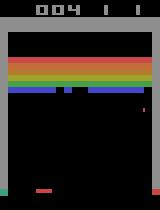
\includegraphics[width=\textwidth]{images/robotfeaturesextractorsequence/robotfeatures-original-image.jpg}
            \end{figure}
    \end{columns}
\end{frame}

\begin{frame}{Robot Features Extraction}
    \begin{columns}[c,onlytextwidth]
        \column{0.7\textwidth}
            \parbox{0.95\textwidth}{
                Considering only the \textbf{upper part} of the\\
                observation which contains the ball.}
        \column{0.3\textwidth}
            \begin{figure}
                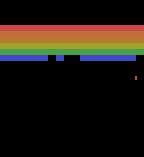
\includegraphics[width=\textwidth]{images/robotfeaturesextractorsequence/robotfeatures-upper-part.jpg}
            \end{figure}
    \end{columns}
\end{frame}

\begin{frame}{Robot Features Extraction}
    \begin{columns}[c,onlytextwidth]
        \column{0.7\textwidth}
            \parbox{0.95\textwidth}{
                \begin{itemize}
                    \item \texttt{inRange} function to consider only pixels with
                        the same color of the ball, obtain a black and white image
                    \item remove the \textbf{remaining bricks} by checking
                        sorrounding pixels, width of the ball is much smaller
                \end{itemize}
            }
        \column{0.3\textwidth}
            \begin{figure}
                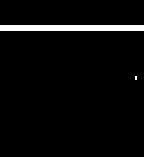
\includegraphics[width=\textwidth]{images/robotfeaturesextractorsequence/robotfeatures-bottom-part-mask.jpg}
            \end{figure}
    \end{columns}
\end{frame}

\begin{frame}{Robot Features Extraction}
    \begin{columns}[c,onlytextwidth]
        \column{0.7\textwidth}
            Determine the position of the ball:
            \begin{itemize}
                \item find \textbf{contours}
                \item extract \textbf{centroid} of the ball
                \item $\text{ball}_x=135, \text{ball}_y=77$
            \end{itemize}
        \column{0.3\textwidth}
            \begin{figure}
                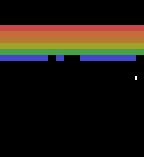
\includegraphics[width=\textwidth]{images/robotfeaturesextractorsequence/robotfeatures-bottom-part-ballposition.jpg}
            \end{figure}
    \end{columns}
\end{frame}

\begin{frame}{Robot Features Extraction}
    \justifying
    Return the difference between the position of the paddle and the ball
    on the $x$ axis and the position of the ball on the $y$ axis:
    \begin{equation*}
        (\text{ball}_x - \text{paddle}_x + 143, \text{ball}_y) = (243, 77)
    \end{equation*}
\end{frame}

\begin{frame}{Goal Features Extraction}
    \begin{columns}[c,onlytextwidth]
        \column{0.7\textwidth}
            \parbox{0.95\textwidth}{
                Extract a binary representation of the bricks from the
                observation:\\
                \begin{equation*}
                    \begin{smallmatrix}
                        1 & 1 & 1 & 1 & 1 & 1 & 1 & 1 & 1 & 1 & 1 & 1 & 1 & 1 & 1 & 1 & 1 & 1 \\
                        1 & 1 & 1 & 1 & 1 & 1 & 1 & 1 & 1 & 1 & 1 & 1 & 1 & 1 & 1 & 1 & 1 & 1 \\
                        1 & 1 & 1 & 1 & 1 & 1 & 1 & 1 & 1 & 1 & 1 & 1 & 1 & 1 & 1 & 1 & 1 & 1 \\
                        1 & 1 & 1 & 1 & 1 & 1 & 1 & 1 & 1 & 1 & 1 & 1 & 1 & 1 & 1 & 1 & 1 & 1 \\
                        1 & 1 & 1 & 1 & 1 & 1 & 1 & 1 & 1 & 1 & 1 & 1 & 1 & 1 & 1 & 1 & 1 & 1 \\
                        1 & 1 & 1 & 1 & 1 & 1 & 0 & 1 & 0 & 0 & 1 & 1 & 1 & 1 & 1 & 1 & 1 & 0 \\
                    \end{smallmatrix}
                \end{equation*}

                It will be used to evaluate fluents in temporal goals.
            }
        \column{0.3\textwidth}
            \begin{figure}
                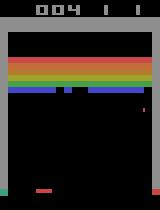
\includegraphics[width=\textwidth]{images/robotfeaturesextractorsequence/robotfeatures-original-image.jpg}
            \end{figure}
    \end{columns}
\end{frame}

\begin{frame}{Temporal Goals}
    \begin{itemize}
        \item string formula to break rows from top to bottom:
    \end{itemize}
        \begin{center}
            \texttt{<(!l0 \& !l1 \& ... \& !l5)*;\\
                    ( l0 \& !l1 \& ... \& !l5); \\
                    ...\\
                   ~( l0 \& ~l1 \& ... \& !l5)*;\\
                  ~~( l0 \& ~l1 \& ... \& ~􏰂l5)>tt}
        \end{center}
    \begin{itemize}
        \item parsed with \texttt{LDLfParser} (\texttt{FLLOAT})
        \item \texttt{LDLfFormula} passed to abstract class \texttt{TemporalEvaluator}
        \item automaton is being created (\texttt{RLTG}, DFA built upon
            \texttt{Pythomata}) in order to create the extended MDP
    \end{itemize}
\end{frame}
